% !TeX root = ../main.tex

\section{Simulación y análisis}

\subsection{Eventos}
Nuestro modelo tiene la característica de alimentarse de
datos externos para simular los efectos climáticos en la generación de
energía, y las variaciones en el consumo de un hogar. Es por eso, que en vez
de utilizar datos producidos aleatoriamente exclusivamente para llevar a cabo
este trabajo, optamos por utilizar fuentes de datos disponibles en internet,
pero que corresponden a casos reales.

En primer, como fuente de datos de clima, utilizamos un dataset de
Kaggle\footnote{\url{https://www.kaggle.com/runphilrun/hi-seas-solar-radiation-prediction}},
una plataforma para abierta para compartir fuentes de datos, y llevar a cabo
competencias en ciencias de datos. Los mismos fueron recolectados por
NASA\footnote{\url{https://hi-seas.org/}}, en dos misiones llevadas a cabo en
una instalación ubicada en la base de un volcán en Hawaii, Estados Unidos. La
expedición es llamada HI-SEAS (\textit{Hawai’i Space Exploration Analog and
Simulation}), y los datos corresponden a las misiones IV y V (septiembre a
diciembre de 2016).

La fuente de datos posee diversas mediciones meteorológicas, pero de estas
solo nos interesa la radiación solar, medida en $\frac{Watts}{m^2}$; y la
velocidad del viento, medida en $\frac{km}{hora}$. Todas estas mediciones
fueron realizadas con una frecuencia de cinco minutos.

Por otro lado, la fuente de datos utilizada para el consumo eléctrico
corresponde a \textit{University of California,
Irvine}\footnote{\url{https://archive.ics.uci.edu/ml/datasets/Individual+household+electric+power+consumption}},
y fueron tomadas en una casa en Francia, entre diciembre de 2006 y 2010. El
dato que extrajimos de esta fuente es la potencia activa consumida, medida
cada un minuto, y cuya unidad es $Watts$. Algo importante a notar, que puede
ser posible gracias a la asincronía que soporta DEVS en los eventos que
suceden, es que $1,25\%$ de las mediciones son nulas (debido a algún
inconveniente en la lectura de las mismas), las cuales fueron omitidas, y por
consiguiente, no incluidas entre los eventos disparados en la simulación.

Los eventos fueron procesados y combinados en un solo archivo de eventos. El
procesamiento consistió en: 
\begin{itemize} 
    \item Conversión de las unidades originales de las fuentes de datos a las
    utilizadas en el modelo.
    \item Normalización de las fechas asignadas a cada medición, para que las
    mismas arranquen en 00:00:00:00 (en tiempo DEVS, el inicio de la
    simulación), y conversión de las mismas al formato de tiempo utilizado
    por el simulador, respetando la diferencia relativa entre los eventos.
    Para esto se tomo la fecha 00:00:00:00 como la hora 00:00 AM, del primer
    día simulado.
    \item Inclusión de ambas fuentes de datos en un mismo archivo de eventos.
    Resultó interesante descubrir que el simulador ignora el orden en el que
    lee los eventos del archivo, ya que después al programarlos para ser
    disparados los reordena, lo cual permite armar el archivo no teniendo que
    ordenar los eventos manualmente.
\end{itemize} % TODO: Descripción cuantitativa de los datos?

\subsection{Elección de generadores}
Para calcular la energía generada por la celda solar, usamos la siguiente formula:

$$producedEnergy = \frac{radiation \times PeakPower \times Area}{1000}$$

Donde $PeakPower$ es un factor que depende del generador.

Buscamos las especificaciones de un equipo\footnote{https://www.fiasa.com.ar/DoWNloADs/FIASA-FOLLETO-GENERADOR-SOLAR.pdf}  
y tomamos uno con $PeakPower=100$. Consideramos entonces un panel solar de 1m$^2$ y con estos valores calculamos la
energía producida por este medio.

Para la turbina eólica buscamos un modelo teórico que explique los valores generados,
pero no lo pudimos ajustar con las especificaciones de turbinas, así que elegimos un
modelos y utilizamos una interpolación de manera que se ajuste a los valores 
provistos por el vendedor. \footnote{https://articulo.mercadolibre.com.ar/MLA-616433420-turbina-generador-eolico-aerogenerador-1200w-48v-enertik-\_JM}

\subsection{Ambiente de Simulación y experimentación} 
El procedimiento que utilizamos para llevar a cabo la simulación y analizar
los datos, consiste en, teniendo el archivo con los eventos procesados,
simular la cantidad de tiempo deseada (una semana en la mayor parte de los
análisis). Luego, utilizando los resultados obtenidos de la simulación
(puertos de salida del \textit{top model}, y logs (no propios de DEVS, sino
instrumentados en el modelos en si) obtenidos de alguna de los modelos), se
realizó un análisis cuantitativo y cualitativo.

Para el análisis de los datos, se utilizo \textit{Jupyter Notebooks}, junto
con diversas bibliotecas de \textit{Python}, tanto para lectura, filtrado y
transformación de los datos; como para graficar y obtener medidas
estadisticas.

\pagebreak
\subsection{Desarrollo}
El desarrollo esta organizado de la manera en la que fueron sucediendo las
simulaciones realizadas (se incluye en cada una las configuraciones pasadas
al simulador, de forma de poder replicarlas fácilmente\footnote{Todos los
comandos son tomando como directorio base:
\textit{TP\_ROOT/simulation/src}.}; y el correspondiente \textit{notebook}\footnote{\texttt{Notebooks/solarVsEolica.ipynb}}
con el análisis). Cada sección tiene algunas conclusiones parciales, y
construye sobre la anterior.

\subsubsection{¿Cuál medio de generación aporta más?}
% ./bin/cd++ -e../eventGeneration/mergedData.ev -mmodels/solarAndWindControllerModel.ma -oout/solarAndWind1Week -lout/solarAndWind1Week.log -t168:00:00:00

    \hypertarget{suxf3lo-generaciuxf3n-solar-1-semana}{%
\subsubsection{Sólo generación solar, 1
semana}\label{suxf3lo-generaciuxf3n-solar-1-semana}}

\hypertarget{comando-ejecutado}{%
\paragraph{Comando ejecutado:}\label{comando-ejecutado}}

\texttt{./bin/cd++ -e../eventGeneration/mergedData.ev
-mmodels/justSolarControllerModel.ma -oout/justSolar1Week
-lout/justSolar1Week.log -t168:00:00:00}

    En esta primera simulación, se evalúa el comportamiento del sistema
completo, pero solo utilizando el panel solar como fuente de generación.

Lo primero que es interesante notar, es como el comportamiento del panel
varía congruentemente con el horario del día, teniendo su pico de
generación cercano al mediodía, y disminuyendo para ambos extremos
(noche y madrugada). Esto muestra cómo con un modelo muy simple, y datos
tomados de su contraparte real, una simulación puede asemejarse mucho al
comportamiento verídico.

Como hay una franja en específico durante la cual el generador produce,
se puede notar cómo la carga de la batería fluctúa, pasando entre los
estados de disponible, en el cual se habilita el consumo de la misma, a
vacía. Esto se debe a que la generación del panel es suficiente para
mantener la carga en la batería, y a la vez, suministrar la demanda
impuesta.

Es posible que, modificando la instalación para que soporte un array de
paneles, en vez de uno solo, la potencia generada crezca linealmente con
la cantidad de ellos. De esta manera, podría soportar la carga, y a la
vez, preservar la carga.

Se puede ver también como los momentos de más generación no se
corresponden los con los de menor consumo, situación en la que el panes
\emph{podría} llegar a abastecer la demanda impuesta, y cargar la
batería en los momentos de mayor consumo (en la que por si mismo, no
realiza mucho aporte).

    \begin{center}
    \adjustimage{max size={0.9\linewidth}{0.9\paperheight}}{secciones/solarVsEolica_files/solarVsEolica_9_0.png}
    \end{center}
    { \hspace*{\fill} \\}
    
    \begin{center}
    \adjustimage{max size={0.9\linewidth}{0.9\paperheight}}{secciones/solarVsEolica_files/solarVsEolica_10_0.png}
    \end{center}
    { \hspace*{\fill} \\}
    
    \hypertarget{suxf3lo-generaciuxf3n-solar-y-euxf3lica-1-semana}{%
\subsubsection{Sólo generación solar y eólica, 1
semana}\label{suxf3lo-generaciuxf3n-solar-y-euxf3lica-1-semana}}

\hypertarget{comando-ejecutado}{%
\paragraph{Comando ejecutado:}\label{comando-ejecutado}}

\texttt{./bin/cd++\ -e../eventGeneration/mergedData.ev\ -mmodels/solarAndWindControllerModel.ma\ -oout/solarAndWind1Week\ -lout/solarAndWind1Week.log\ -t168:00:00:00}

    En esta segunda simulación, se evalúa el mismo sistema, pero con ambos
generadores.

Se puede ver la gran diferencia en la carga y la generación de ambas
simulaciones. El aporte de la turbina eólica hace que el comportamiento
del SmartGrid cambie radicalmente, pudiendo sumistrar la totalidad de la
energía solicitada por intervalos extensos.

También se puede ver como a diferencia de la batería, en los instantes
de menos consumo el sistema alcanza a soportar la totalidad del consumo
de la instalación, produciendo un ahorro considerable (proyectando el
mismo comportamiento a un mes, por ejemplo).

Hay momentos en los cuales la batería se encuentra llena, y permanece de
esa manera durante un tiempo. Aquí surgen dos alternativas: - Vender la
energía excedente que esta siendo generada, lo cual es la ida central de
un SmartGrid. - Aumentar la capacidad de la batería, de manera de
cargarla aún más, y autoabastecer la instalación por instantes de timpo
aún mayores.

De ambas formas se produce un ahorro. Se podría establecer el costo de
cada opción, y mediante simulaciones como esta (con alguna pequeña
diferencia en los modelos) concluir cual es la más viable.

    \begin{center}
    \adjustimage{max size={0.9\linewidth}{0.9\paperheight}}{secciones/solarVsEolica_files/solarVsEolica_14_0.png}
    \end{center}
    { \hspace*{\fill} \\}
    
    \begin{center}
    \adjustimage{max size={0.9\linewidth}{0.9\paperheight}}{secciones/solarVsEolica_files/solarVsEolica_15_0.png}
    \end{center}
    { \hspace*{\fill} \\}
    
    \hypertarget{quuxe9-generador-vale-muxe1s}{%
\subsubsection{Qué generador vale
más?}\label{quuxe9-generador-vale-muxe1s}}

    Si vemos cuánto generaron en cada instante ambos generadores de manera
acumulada, lo primero que podemos notar es la variabilidad de los
valores. Hay instantes en los que la potencia acumulada llega a los
\(650W\), mientras que al momento siguiente llega a casi 0. A priori uno
pensaría que esto se debe a los datos, lo cual es en parte cierto, pero
el problema va más alla de eso. Como ambos generadores varían su
potencia generada al recibir como evento un cambio en el estado
meteorólogico de la simulación, de manera instantánea, esto da lugar a
ciertas situaciones especiales, dadas por la forma en la que se
realizaron las mediciones utilizada como eventos: - Si en algún momento
el instrumento para medir la radiación solar fue ocluído, esto dará
lugar a una serie de mediciones en las cuales su valor disiminuyo
significativamente, no representando la realidad. - Cambios repentinos
en la velocidad del viento, lo cual es normal, ya que el mismo puede
tener un comportamiento compuesto por ráfagas. - Problemas en los
instrumentos, lo cual dará mediciones erróneas, o valores no
consistentes.

Pero más allá de esto, esto podría solucionarse si los modelos de los
generadores tuvieran algún tipo de inercia. Esto sería, algún tipo de
resistencia al cambio repentino, no viendose su salida, o su estado
interno afectado por que de un instante para el otro se recibió un
evento qué indicaba que la velocidad del viento disminuyó a casi cero, y
depués de este otro en el cual ya volvió al valor anterior (tomando como
ejemplo el generador eólico). Aparte, el generador eólico es un caso
especial, ya que físicamente poseé inercia (si su rotor está girando a
una velocidad \(V > 0\), el que la velocidad del viento disminuya a cero
no hará que \(V\) pase a valer cero en el acto).

    \begin{center}
    \adjustimage{max size={0.9\linewidth}{0.9\paperheight}}{secciones/solarVsEolica_files/solarVsEolica_18_0.png}
    \end{center}
    { \hspace*{\fill} \\}

    Si omitimos estas consideraciones, igual podemos notar la diferencia
entre la potencia producida por el generador eólico y el solar. No solo
en la intensidad de la misma, sino en la constancia.

Por otro lado, como la fuente de energía del generador eólico no depende
del horario del día (al menos no de manera directa), tiene un
comportamiento mucho mas constante, generando valores parecidos en
cualquier instante.

Si normalizamos los valores de producción de energía en cada instante,
podemos ver qué porcentaje de lo generado corresponde a cada uno de los
generadores. Como era de esperar, gran parte corresponde a la turbina
eólica, cubriendo en promedio el \(83,16\%\) de la energía producida.
Más alla de esto, hay insttante en que casi la totalidad de la
generación corresponde al panel solar. Esto puede deberse a los
problemas descriptos anteriormente, pero hay instantes en los que por
alrededor de una hora la velocidad del viento disminuyó
significativamente, que pueden dar sentido a las observaciones.

    \begin{center}
    \adjustimage{max size={0.9\linewidth}{0.9\paperheight}}{secciones/solarVsEolica_files/solarVsEolica_21_0.png}
    \end{center}
    { \hspace*{\fill} \\}


\subsection{Consumo acumulado:}
A continuación observaremos las señales enviadas desde el controlador a la red, graficando
como positivas las señales de pedido de energía por parte de la red, y como negativas las
de venta de energía a la red.

El tiempo considerado es de una semana y la energía solicitada/pedida se mide en Watts hora.

\begin{figure}[H]
    \centering
    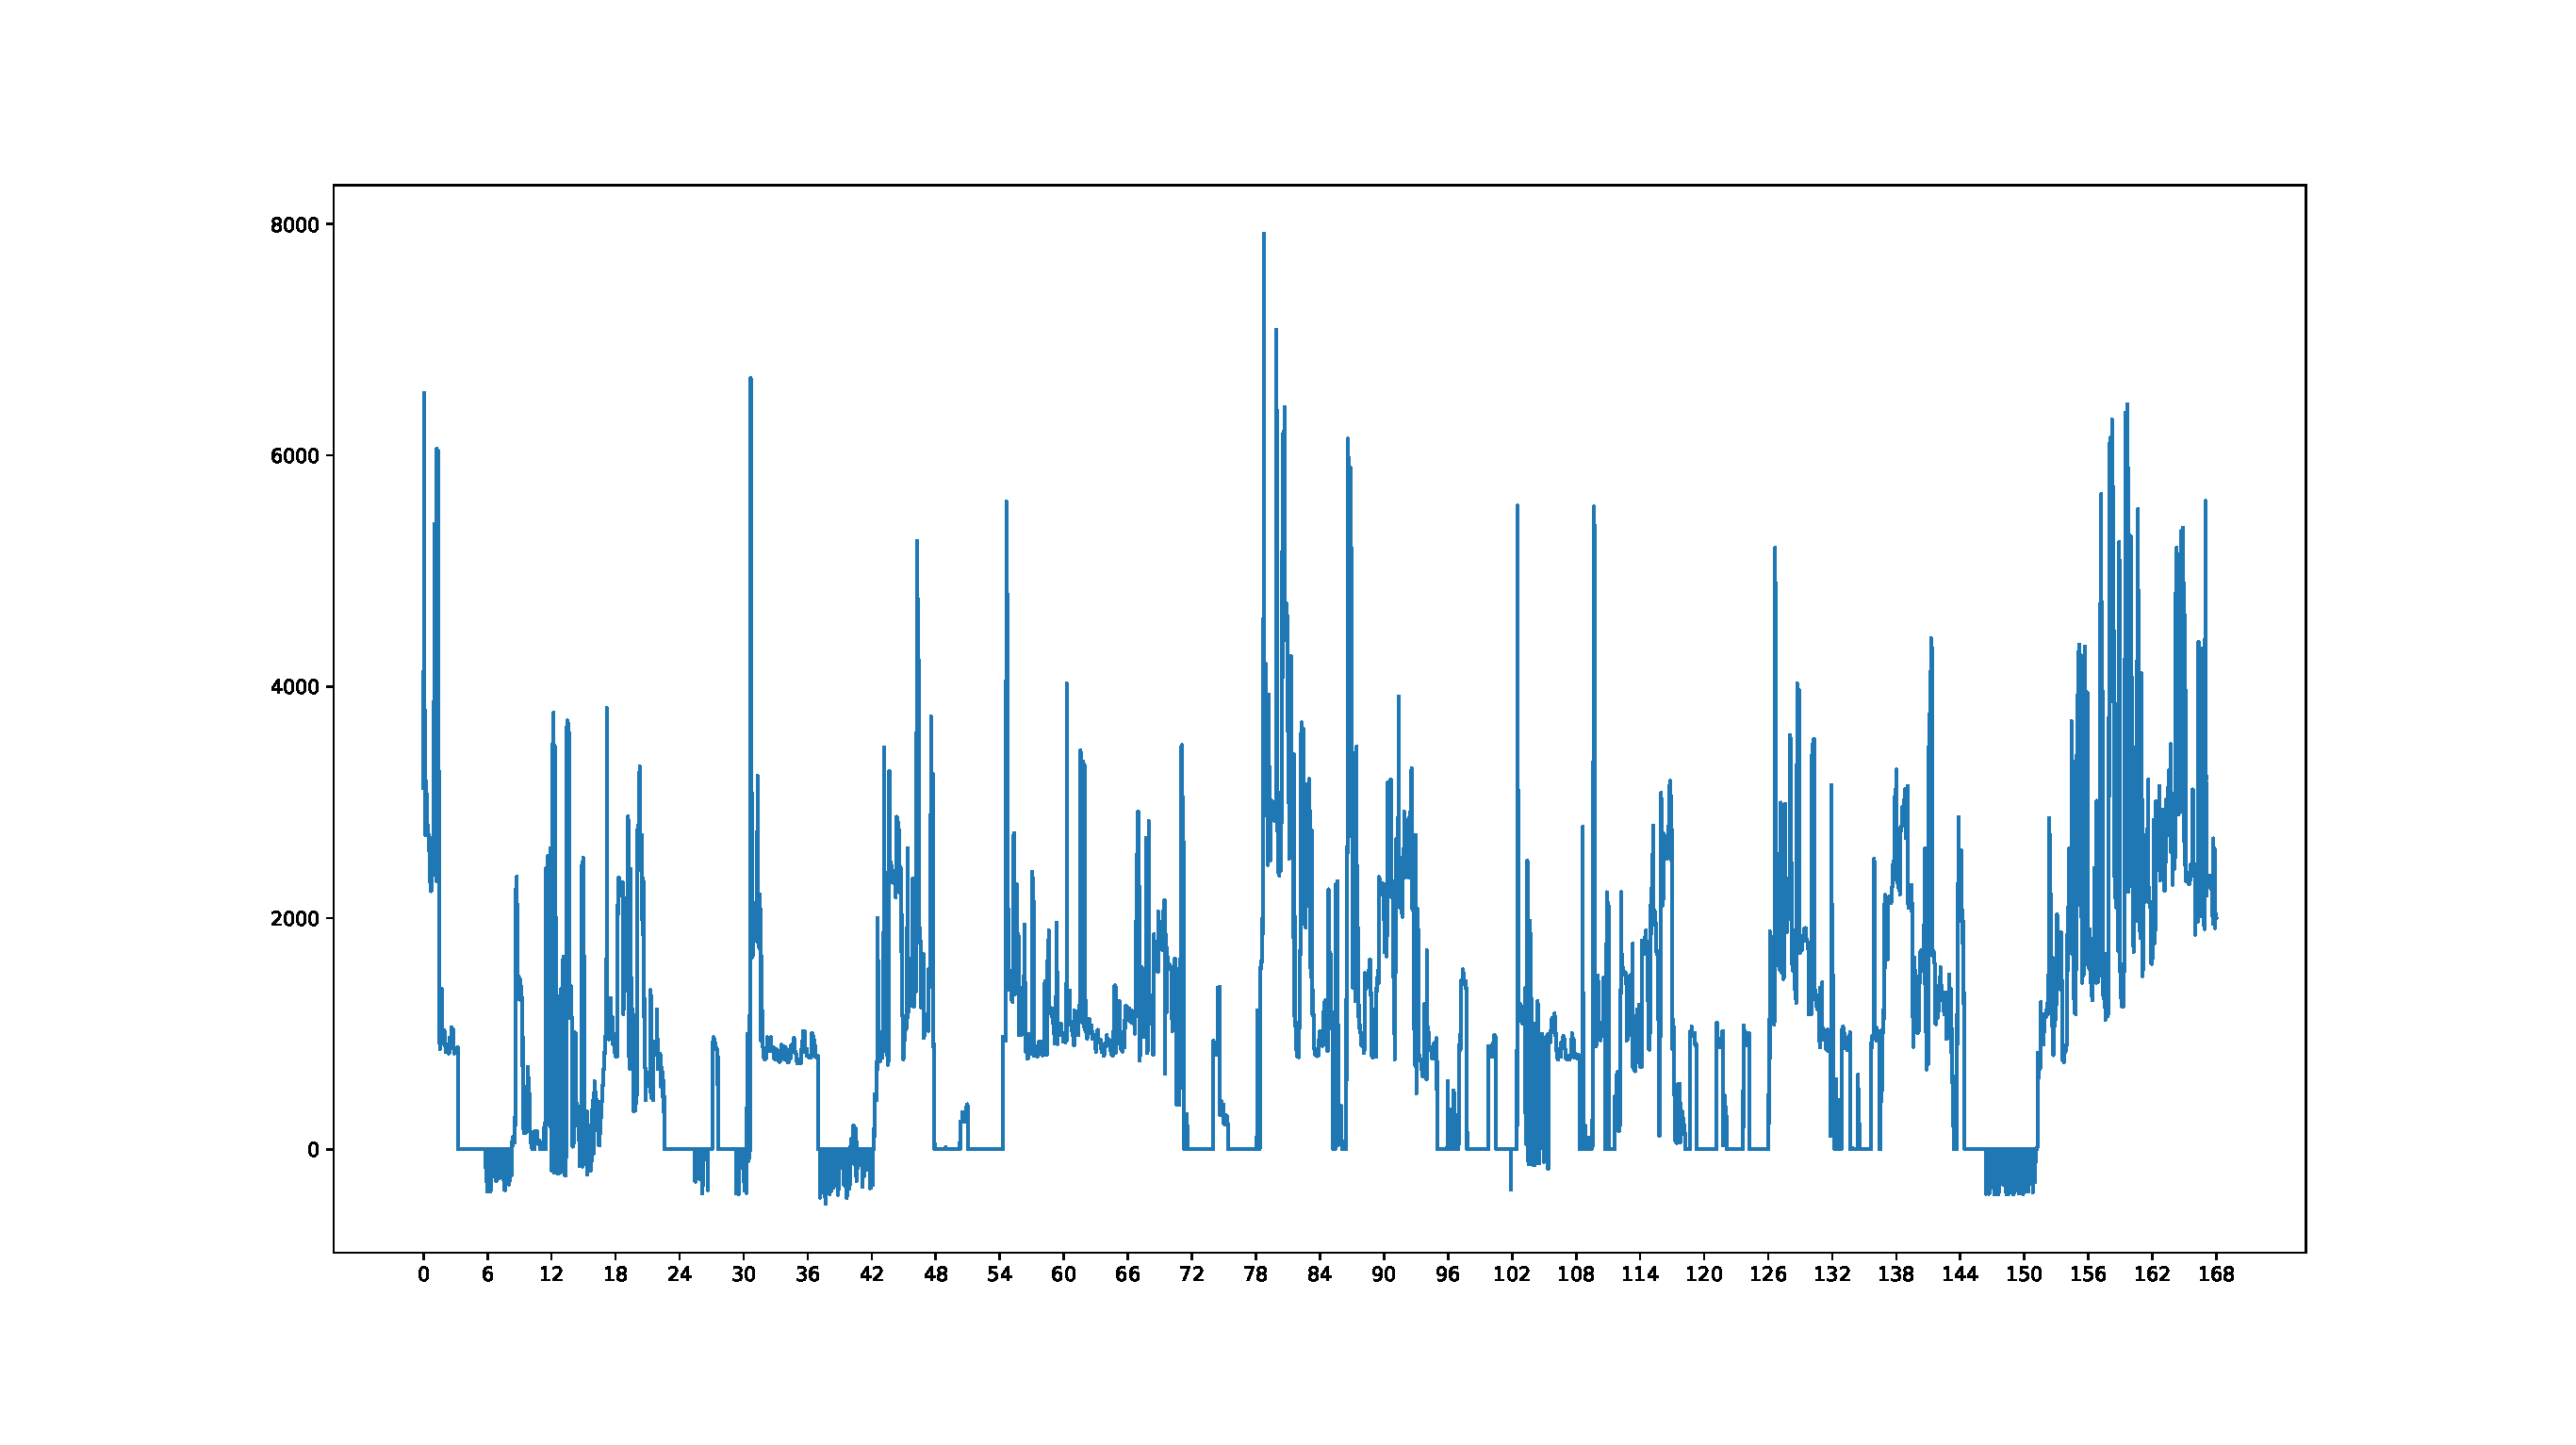
\includegraphics[scale=0.3]{images/cons.eps}
\end{figure}

Ahora calculamos el acumulado de estos valores podemos observar como evoluciona el
balance de energía. 

\begin{figure}[H]
    \centering
    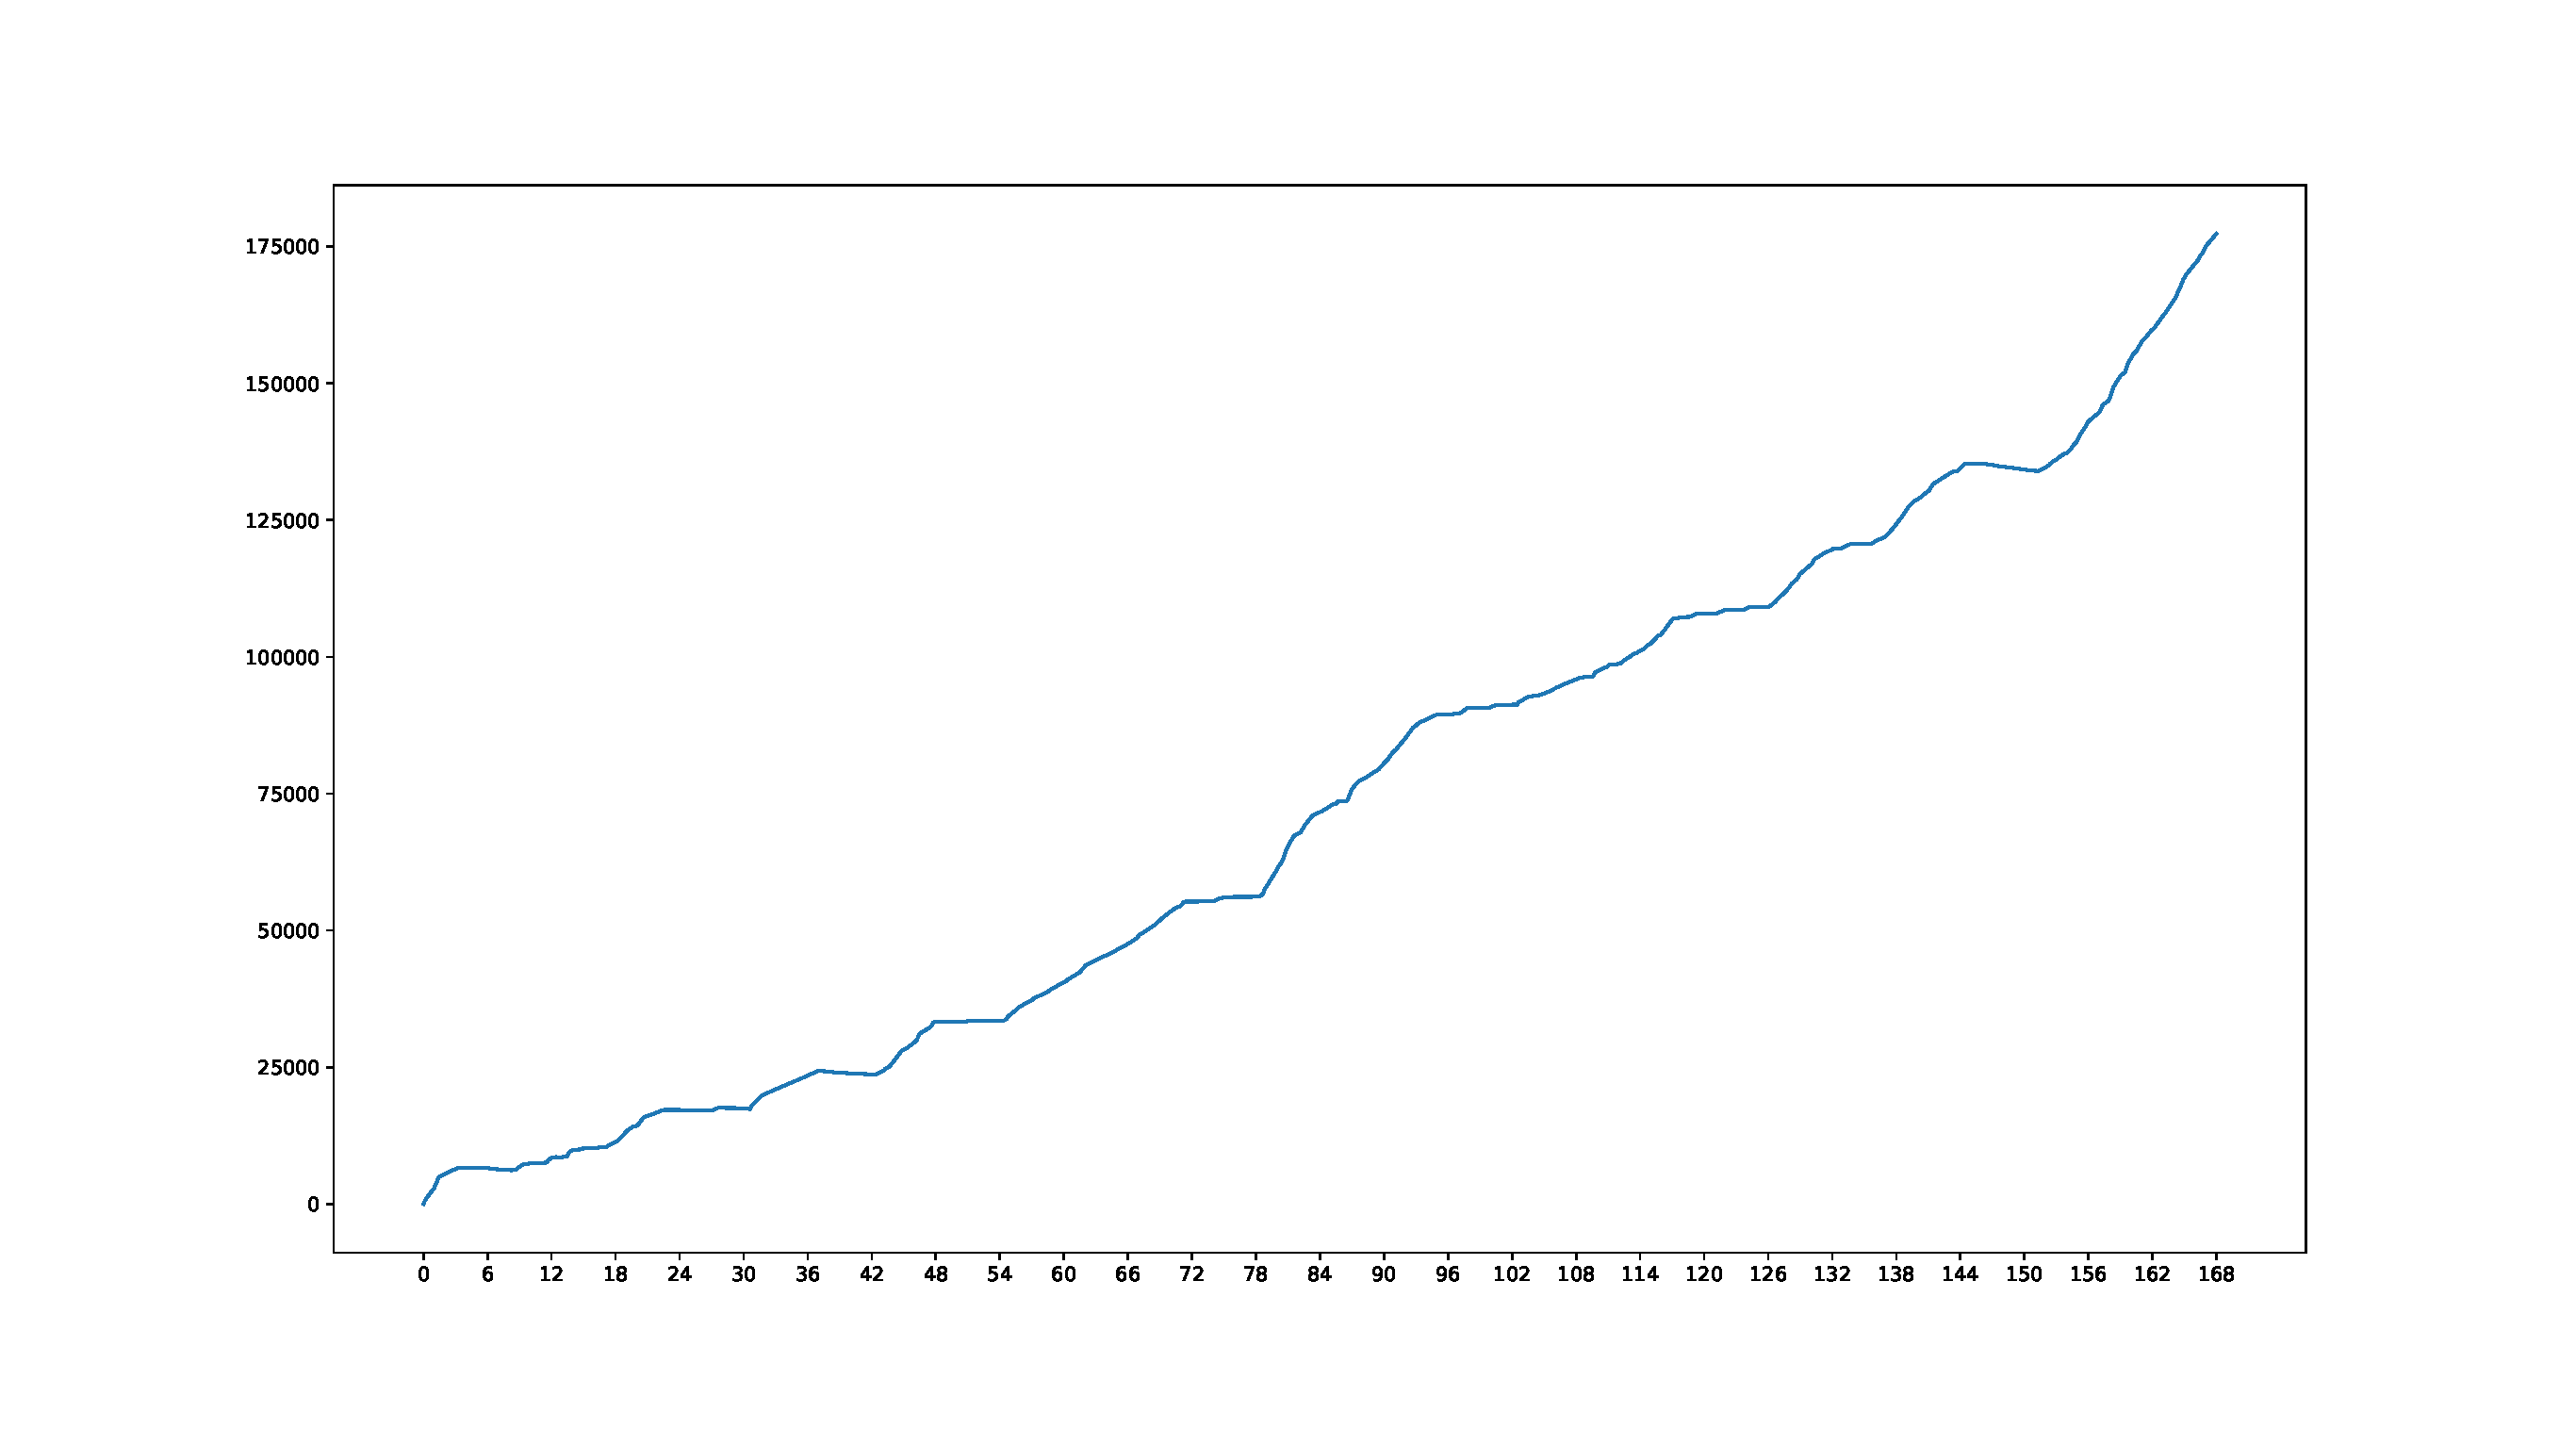
\includegraphics[scale=0.3]{images/acc.eps}
\end{figure}

En el gráfico vemos que con estos generadores aún existe bastante dependencia de la red,
pero el consumo de una semana es mucho menor (175kW).